%!TEX root = ../main.tex

\par
After an Atlantic hurricane dissipates, the National Hurricane Center (NHC) determines the most accurate track of the storm, and collects various other information about the storm throughout its lifetime.
Both modern and historical data have been combined to produce a database containing information on every single Atlantic hurricane since 1851, known as the revised Atlantic hurricane database, or HURDAT2~(\cite{landsea2015revised}).
The available data includes information about the hurricane taken every six hours, from the formation of the storm to its dissipation.
This includes:
\begin{itemize}
	\item Latitude and longitude of the system center
	\item Landfall events
	\item Maximum sustained wind
	\item Minimum barometric pressure
	\item Maximum extent of hurricane and tropical storm winds
\end{itemize}

\par
On occasion, there will be additional measurements besides the six hour updates, to mark important events in the storm's lifetime.
For example, the data for Hurricane Irene (from 2011) contains an entry at 9:35 AM on August 28 to indicate a landfall that occurred at that time.
Another example is Hurricane Gordon (from 2018); the dataset contains an entry at 9:00 AM on September 3 to provide additional detail on the intensity of the storm during a period of time where that intensity is rapidly changing.

\par
The tracked latitude and longitude of the system center is one very important component of the dataset, as it allows us to examine the path a hurricane has taken throughout its lifetime.
It also implicity gives us information on where the hurricane formed, and can be used to compare different storms to see how similar they are.
For these reasons, the track of a hurricane is the most useful information to us, and will be the variable we focus on for prediction.

\par
The maximum sustained wind and minimum batrometric pressure are two pieces of information that can be helpful for tracking how powerful a hurricane is.
Both represent the peak strength of a hurricane at a given time, albeit in different ways.
Maximum sustained wind speed and minimum barometric pressure are direct measurements of the power of a storm.
In addition, the change in barometric pressure indicates whether a storm is strengthening or weakening.
However, the focus of this paper is primarily predicting whether or not a storm will landfall, so the strength of historical storms is only tangentially relevant.

\par
The extent of hurricane and tropical storm winds for a given hurricane gives us valuable information about how large a storm is.
In addition, because those measurements are separated by the quadrant of the storm, they provide knowledge of the shape of the storm.
Utilizing this information to improve my predictions could be successful, but it is beyond the scope of this paper.

\begin{figure}
	\centering
	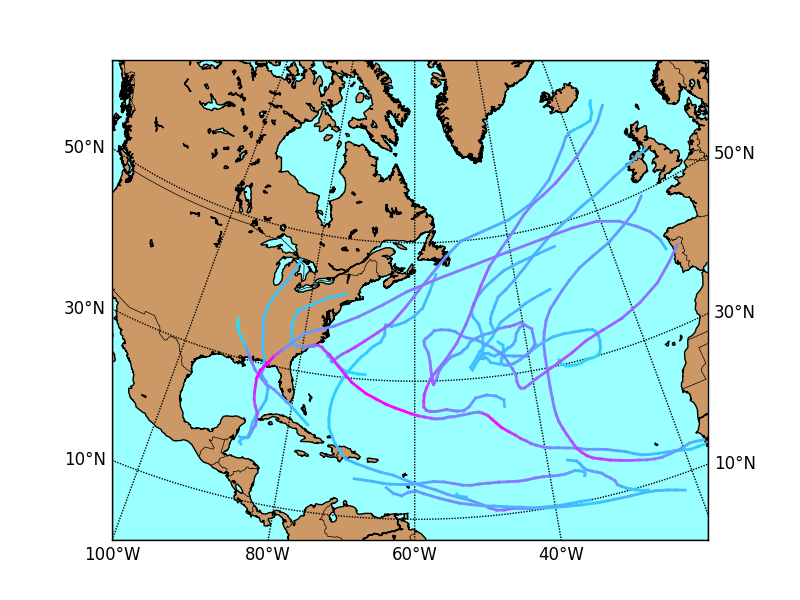
\includegraphics[width=\linewidth]{images/2018_max_winds.png}
	\caption{A map of the track of every Atlantic tropical storm in 2018. The color represents the maximum wind speed of the hurricane at that point in time -- magenta being the most intense.}
	\label{fig:2018_storm_tracks}
\end{figure}

\par
Finally, tracking whether or not a hurricane made landfall, and the conditions when it made landfall, allows us to esimate how dangerous the hurricane was.
A strong hurricane which never makes landfall is much less hazardous than a weak hurricane that does.
I will specifically use this information as the dependent variable when training my statistical models.

% \begin{figure}
% 	\centering
% 	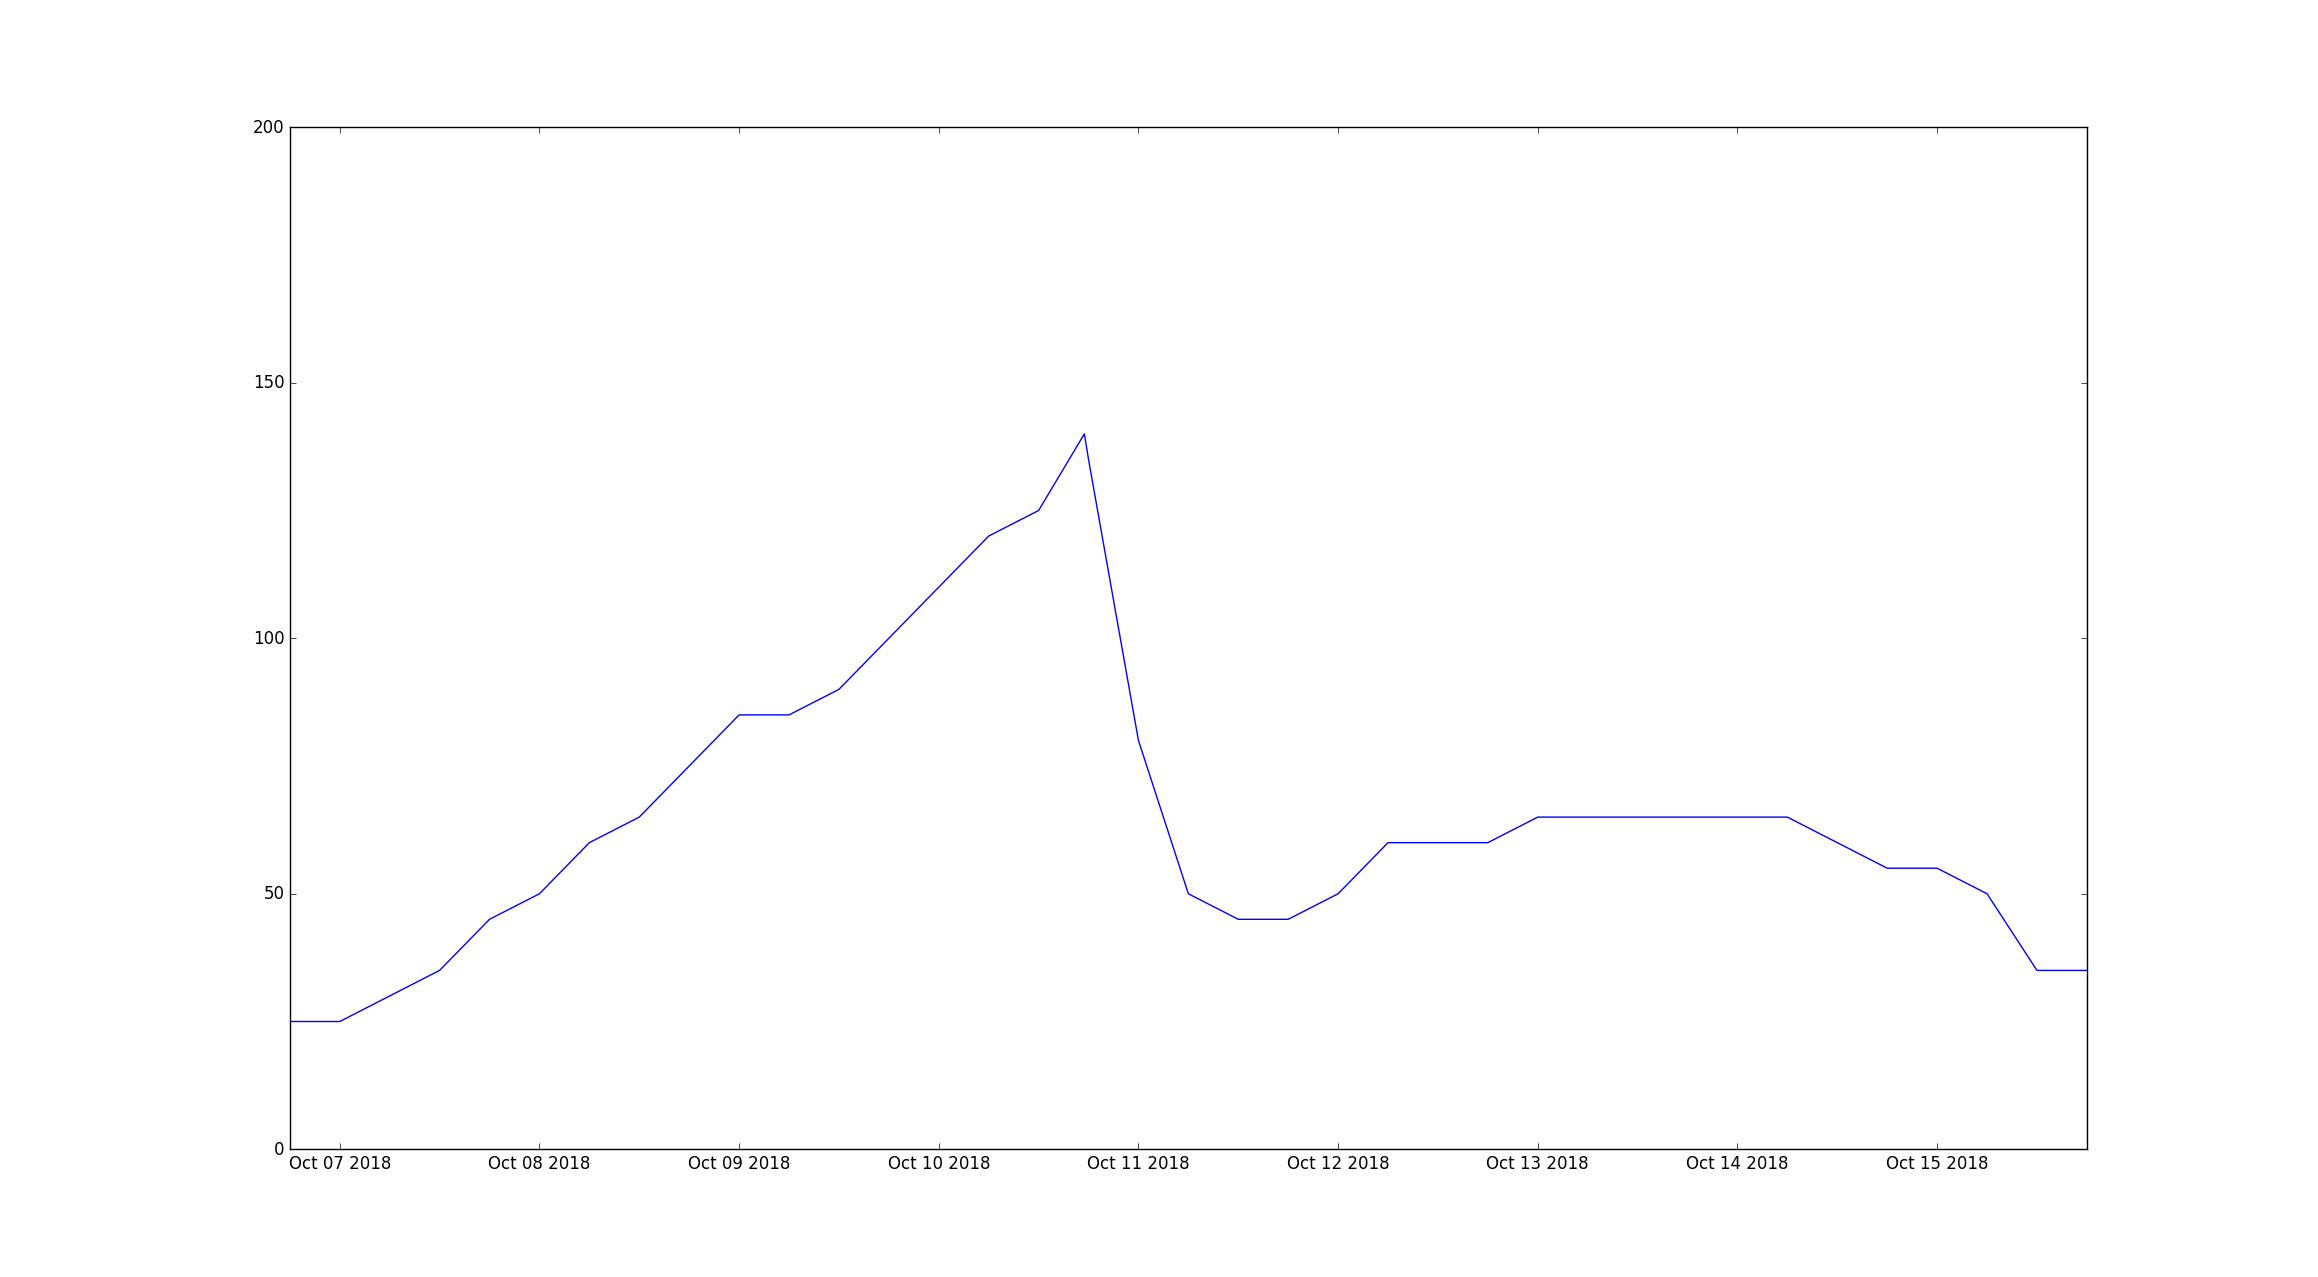
\includegraphics[width=\linewidth]{images/hurricane_michael_max_wind.png}
% 	\caption{A plot of the maximum wind speed of Hurricane Michael over its lifetime.}
% \end{figure}

\subsection{High-Level Analysis}

\par
Figure~\ref{fig:2018_storm_tracks} plots the track of every Atlantic hurricane in 2018, in order to demonstrate the most common paths for hurricanes to take.
The majority of storms form off the west coast of Africa, initially move west across the Atlantic, then gradually turn north, and eventually back east.
Depending on how this change occurs, and where exactly the storm formed, there are several common outcomes.
Some storms turn to the north early and remain in the mid-Atlantic.
Others turn later, moving up the Atlantic coast.
The remaining hurricanes pass into the Gulf of Mexico before turning north towards the Gulf Coast and continental United States.
There are also some storms which form within the Carribean or Gulf of Mexico -- they tend to move north-northeast towards the United States.

\par
\textcolor{blue}{\textbf{TODO: More misc high-level analysis?}}

\subsection{Using the Data}

\par
As a part of constructing the HURDAT2 database, its creators took the time to examine historical records to ensure that the dataset is as complete as possible.
There are no empty cells in the track data, which means all historical track data is usable without requiring any sort of interpolation.
There are some empty cells in other variables, such as barometric pressure and wind speed extent, but this information is not relevant to this paper's analysis.
Historical research is currently in progress to attempt to find some of these values, but ultimately, some measurements just don't exist.